% *********************************************************************
% © 2021-2022 Jeremy Sylvestre
%
% Permission is granted to copy, distribute and/or modify this document
% under the terms of the GNU Free Documentation License, Version 1.3 or
% any later version published by the Free Software Foundation; with no
% Invariant Sections, no Front-Cover Texts, and no Back-Cover Texts. A
% copy of the license is included in the appendix entitled “GNU Free
% Documentation License” that appears in the output document of this
% PreTeXt source code. All trademarks™ are the registered® marks of
% their respective owners.
%
% *********************************************************************

\newcommand*{\xmin}{-0.1}
\newcommand*{\xmax}{1.25}
\newcommand*{\ymin}{-0.5}
\newcommand*{\ymax}{4.5}

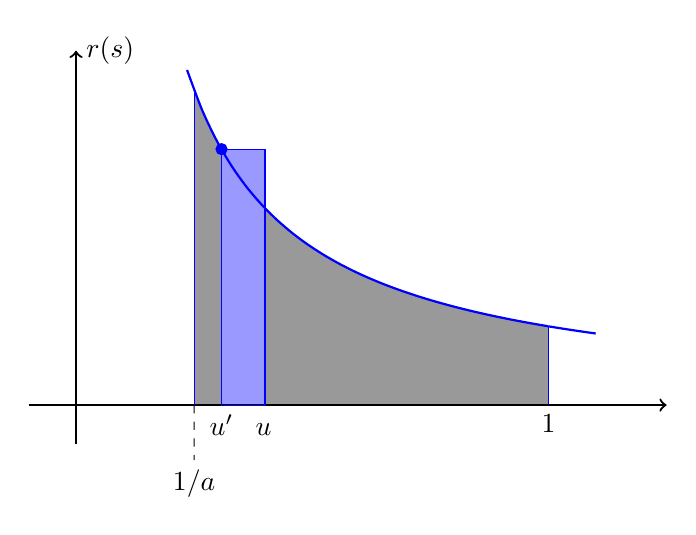
\begin{tikzpicture}
[
	closedpt/.style={circle,draw,fill,inner sep=0pt,minimum size=4pt},
	openpt/.style={circle,draw,inner sep=0pt,minimum size=4pt},
	xscale=6
]


	% fills
	\fill[black!40!white] (0.25,4) plot[domain=0.25:1] (\x,{1 / \x}) -- (1,0) -- (0.25,0) -- cycle;
	\fill[blue!40!white] (0.4,0) rectangle (0.308,3.25);

	% axes
	\draw[->,thick] (\xmin,0) -- (\xmax,0);
	\draw[->,thick] (0,\ymin) -- (0,\ymax) node[right] {$r(s)$};

	% graph
	\draw[thick, blue, domain=0.235:1, smooth] plot (\x,{1 / \x});
	\draw[thick, blue, domain=1:1.1, smooth] plot (\x,{1 / \x});
	\draw[blue] (1,1) -- (1,0);
	\node[below] at (1,0) {$1$};
	\draw[blue] (0.25,4) -- (0.25,0);
	\node at (0.25,-1) (a) {$1 / a$};
	\draw[dashed] (0.25,0) -- (a);

	% slice
	\node[below] at (0.4,0) (u) {$\,u\phantom{'}$};
	\node[below] at (0.308,0) (up) {$u'$};
	\node[blue,closedpt] at (0.308,3.25) (sample) {};
	\draw[blue] (0.4,0) rectangle (0.308,3.25);

	%\draw ($ (sample) - (0.3,0) $) -- ($ (sample) - (0.6,0) $);
	%\draw[<->] ($ (sample) - (0.45,0) $) -- node[left] {$r(s)$} ($ (sample) - (0.45,0.364) $);
	%\draw[<->] ($ (sample) + (-0.1,0.1) $) -- node[above] {$ds$} ($ (sample) + (0.1,0.1) $);

\end{tikzpicture}
